Für unseren temporalen Algorithmus (siehe Abschnitt \ref{ch:Temporaler Algorithmus}) gibt es einen 
wichtigen \nameref{ch:Content2:sec:Retargeting} Schritt.
In diesem Schritt wird eine vorberechnete Textur verwendet. Diese speichert eine
Permutation, die unsere \nameref{ch:Content1:sec:blue noise} Textur vom Bild t in eine
blue noise Textur von Bild t+1 umwandelt. Diese Permutation wird 
dann auf die Startwerte angewandt bevor das nächste Bild t+1 gerendert wird (siehe auch Übersicht \nameref{pic:Render Graph}).
Dadurch werden die blue noise Umverteilungen der \nameref{ch:Content2:sec:Sorting} Phase akkumuliert. 
All diese Vorberechnungen sind möglich, da wir mit \textit{\glqq nur\grqq} quasi-zufälligen Sequenzen 
(siehe Abschnitt \ref{ch:Content1:sec:Quasi-Zufallsfolgen}) arbeiten.
Das andauernde Permutieren von Pixeln bis zu einem Punkt, an dem ein Bild aussieht wie das Andere ist 
ein klassisches TSP, wofür es aktuell keine effiziente optimale Lösungsmethode gibt.
Da wir nur an einer sehr guten Lösung, nahe dem globalen Optimum, interessiert sind 
greifen wir wie in \cite{hal02158423} vorgeschlagen auf das heuristische Approximationsverfahren,
dem Simulated Annealing, zu.

\subsubsection{Allgemein}

Angelehnt an metallurgischem Aufheizen und dem sich anschließenden Abkühlen wollen wir eine approximativ
optimale Lösung finden. Wir haben also eine zu Anfang hohe Temperatur, welche durch eine Abkühlfunktionen
(siehe Abschnitt \ref{subsec:Abkühlfunktion} für Weiteres) verringert wird.
Wir definieren die Energie als pixelweisen Unterschied der sich in Abkühlung 
befindlichen bereits permutierten Textur und der $Textur_{t+1}$(siehe Abbildung \ref{eq:pixel energy function}). 
$Textur_{t+1}$ ist durch quasi Zufall (siehe Abschnitt \ref{ch:Content1:sec:Quasi-Zufallsfolgen}) bereits bekannt.
Mit Erkenntnissen aus\cite{georgiev2016blue} ergibt sich

\begin{figure}[H]
  \[ E(SA) = \sum_{p \neq q}E(p,q) = \sum_{\forall i \in [0,N-1]} \Vert{p_{i}-q_{i}}\Vert \]
  \caption{\nameref{ch:Content1:sec:blue noise} Textur mit Dimension N; Pixel p von abkühlende 
  $Textur_{t=0}$; Pixel q von $Textur_{t=1}$}
  \label{eq:pixel energy function}
\end{figure}

Mit dem definierten Ziel, die Energiefunktion \ref{eq:pixel energy function} zu minimieren, wenden 
wir in jedem Schritt eine Permutation an und entscheiden anhand einer Akzeptanzwahrscheinlichkeitsfunktion
\ref{eq:Akzeptanzwahrscheinlichkeitsfunktion}, ob wir diese Permutation beibehalten.
Da wir in jedem Schritt nur eine Permutation anwenden, vereinfacht sich unsere Energiefunktion
\ref{eq:pixel energy function} zu 

\newpage

\begin{figure}[H]
  \[ E(SA) = E(s_{previous}) + \Vert{p_{i}-q_{i}}\Vert + \Vert{p_{i 
        + permutation}-q_{i + permutation}}\Vert\]
  \caption{Zustand $s_{previous}$ ohne angewandte Permutation}
  \label{eq:vereinfachte pixel energy function}
\end{figure}


\begin{figure}[H]
    \centering
    \begin{subfigure}[b]{0.4\textwidth}
        \begin{equation}\label{eq:Akzeptanzwahrscheinlichkeitsfunktion}
            P = e^{-(\Delta_{energy})/ temperature}
        \end{equation}
        \caption{Akzeptanzwahrscheinlichkeitsfunktion; Abhängig von Energie und aktueller Temperatur}
    \end{subfigure}
    ~ %add desired spacing between images, e. g. ~, \quad, \qquad, \hfill etc. 
      %(or a blank line to force the subfigure onto a new line)
    \begin{subfigure}[b]{0.7\textwidth}
        \centering 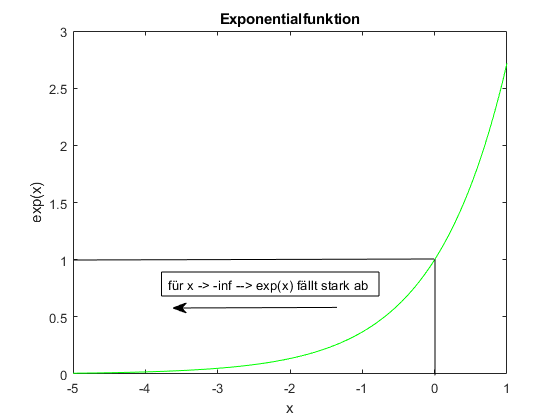
\includegraphics[interpolate=false,width=\linewidth]{content/simulatedAnnealing/Bilder/exponentialfunktion_as_PDF.png}
        \caption{Günstige Eigenschaft der Exponentialfunktion}
        \label{fig:Exponentialfunktion}
    \end{subfigure}
    \caption{}
\end{figure}

Die günstigen Eigenschaften der Exponentialfunktion (siehe Abbildung \ref{fig:Exponentialfunktion}) als
Wahrscheinlichkeitsakzeptanzfunktion sind vielfältig und bereits in weiterführender Literatur wie 
\cite{Kirkpatrick671},\cite{van1987simulated} gut belegt. Eine der Eigenschaften ist in der obigen Abbildung 
\ref{fig:Exponentialfunktion} dargestellt. Das Argument der Funktion \ref{fig:Exponentialfunktion} hat 
einen Divisor Temperatur und einen Dividenten $\Delta_{energie}$.
Mit absteigender Temperatur erkennt man 
in der Abbildung \ref{fig:Exponentialfunktion} eine ebenfalls abnehmende Wahrscheinlichkeit
der Akzeptanz. Dies führt zu dem gewünschten Verhalten, energiehöhere Zustände 
zuzulassen, um somit lokale Maxima zu verlassen. Dies geschieht bei höheren 
Temperaturen häufiger wohingegen bei niederen Temperaturen ein gefundenes Maxima
seltener verlassen wird. Höhere Deltas führen passender Weise zu einem höheren negativen 
Exponenten und damit eine geringere Akzeptanz als Energiezustände, die nur bisschen 
drüber liegen. Die Wahl des Abkühlvorgangs (also das Updaten der Temperatur über die Zeit)
ist problemspezifisch \cite[S. 9]{Kirkpatrick671}. Dabei muss der Abkühlvorgang derart
gewählt werden, sodass kein bloßer Greedy-Algorithmus entsteht und man in einem lokalen 
Maxima stecken bleibt aber auch kein wahlloses Vertauschen entsteht. Diese Vorgänge habe 
ich im Abschnitt \ref{subsec:Abkühlfunktion} untersucht.
Nun haben wir alle Begriffe zusammen um einen ersten Blick auf den Algorithmus zu werfen.

\begin{algorithm}[H]
    \caption{\textbf{Simulated Annealing}}
    \begin{algorithmic}[1]
        \State initialisiere Startzustand $s=s_{0}$
        \State initialisiere Starttemperatur $T_0$
        \For{i=1...maxSteps}
        \State update Temperatur $t_i$ anhand des Abkühlplans
        \State //Radius für Nachbarschaftssuche ist auf 6 festgesetzt
        \State $s_{neu}\leftarrow$Nachbarzustand(s) //wende hier die Permutation an!
        \State $energy\Delta = energy(s_{neu}) - energy(s)$
        \If{$energy\Delta < 0$}
        \State s = $s_{new}$
        \Else{}
        \If{P(Energie(s), Energie($s_{new}$), temperature)$\ge$ random(0,1)} 
        \State s = $s_{new}$
        \EndIf
        \EndIf
        \EndFor
        \State return Endzustand s;
    \end{algorithmic}
    \label{alg:retargeting}
\end{algorithm}

Für die abzuspeichernde Permutation gilt Folgendes.
Als Startzustand $s_{0}$ definieren wir eine Permutation, die alle 
Elemente auf sich selbst abbildet.
Um von einem Zustand s zu einem neuem Zustand $s_{new}$ zu kommen,
definieren wir eine Nachbarschaftsfunktion \textit{Nachbarzustand()}. 
Diese kann zwei Elemente genau dann vertauschen, wenn Sie in einem 
gegenseitigen Radius r = 6 erreichbar sind(folgend der Empfehlung aus \cite[S.7]{hal02158423})
Dabei vertauschen wir in jedem Schritt ein Pixelpaar. 
Die Wahrscheinlichkeitsfunktion zur neuen Zustandsannahme
P(Energie(s), Energie($s_{new}$)) beschreibt, ob wir den neu
gewählten Zustand $s_{new}$ übernehmen. Dabei wird klassischerweise die
Akzeptanz von Zuständen mit höherer Energie immer kleiner.(bzw. die 
Toleranz gegenüber größeren Fehlern im Bezug zur Zeit). Die allgemeine Akzeptanz von 
Zuständen mit höherer Energie ist dabei von fundamentaler Bedeutung.
Somit verlassen wir möglicherweiße nur lokale Maxima.

\subsection{Abkühlfunktion}
\label{subsec:Abkühlfunktion}

Für die Wahl unserer Abkühlfunktion bieten sich einige Möglichkeiten.(siehe Abbildung \ref{pic:Cool Down Comparisson}).
Im Folgenden wird auf die verschiedenen möglichen Abkühlfunktionen (\cite{ScienceDirectCoolingSchedule}) und ihre Eigenschaften
sowie die Wahl interner Parameter(z.B. Starttemperatur, Gleichgewicht) eingegangen. Denn diese Funktion
trägt maßgeblich mit ihrem Konvergenzverhalten zur Effizienz des Abkühlvorgangs bei.
So beeinflusst Sie auch unsere wichtige Wahrscheinlichkeitsakzeptanzfunktion \ref{eq:Akzeptanzwahrscheinlichkeitsfunktion}.
Nach \cite{Kirkpatrick671} wählen wir die Anfangstemperatur $T_0$ derart, dass anfangs jede Neue generierte Lösung akzeptiert
wird. Außerdem werden wir einen Zustand des Quasiequilibriums (Gleichgewicht) definieren.
Für einige Abkühlvorgänge wird es sinnvoll sein, erst nach einer bestimmten Anzahl von erfolgreichen Zustandsübergängen 
die Temperatur zu senken. Dazu beim jeweiligen Vorgang mehr.

\subsubsection{Hajek}

\begin{equation}\label{eq:Hajek}
    f(t) = T_0\log(1+t)
\end{equation}

In \cite{hajek1988cooling} haben wir eine Abkühlfunktion gegeben, welche durch ihre Eigenschaft,
stets gegen das globale Maximum zu konvergieren, eine Funktion die unter allen Anderen heraussticht.
In Abbildung \ref{pic:Cool Down Comparisson} angedeutet und in weiteren Beobachtungen bestätigt hat sich 
allerdings auch ihre sehr langsame Konvergenz.
Sie hat sich daher für diese Aufgabenstellung als nicht nützliche Abkühlfunktion herausgestellt.

\subsubsection{Linear}

\begin{equation}\label{eq:lineare Abkühlung}
    f(t) = T_0 - \mu*t
\end{equation}
Typische Werte für $\alpha$ liegen zwischen 0.8 and 0.99. Wie man in Abbildung \ref{pic:Cool Down Comparisson}
erkennen kann, ist das Problem der linearen Abkühlung die extreme Langsamkeit.
Anstatt nur am Anfang schlechtere Energiezustände zuzulassen um lokale Minima zu verlassen 
geht der Algorithmus durch diesen Abkühlvorgang in ein bloßes randomisiertes Tauschen von Pixeln über.

\subsubsection{Exponential}
Ist nach \cite{Kirkpatrick671} eine für viele Fälle zutreffende und zu wählende Abkühlfunktion.
Wobei $\alpha \in [0.8; 0.99]$.

\begin{equation}\label{eq:Exponential}
    f(t) = T_0*pow(\alpha,t)
\end{equation}

Wie in Abbildung \ref{pic:Cool Down Comparisson} zu erkennen haben wir hier hingegen zu den vorherigen Vorgängen
eine deutlich schnellere Abkühlung. Jedoch lässt sich hier das andere Extrem, im Vergleich zum bloßen randomisierten
Vertauschen von Pixelpaaren, erkennen: Wir verharren viel zu kurz in einem Temperaturzustand, geraten daher schnell 
in einen \textit{greedy} Zustand und manche Bildbereiche bleiben in einem lokalen Minima hängen.

\subsubsection{Inverse}

\begin{equation}\label{eq:Inverse}
    f(t) = T_0 / (1 + alpha * step)
\end{equation}

Wie in Abbildung \ref{pic:Cool Down Comparisson} zu erkennen haben wir hier hingegen zu ersten beiden Vorgängen
eine deutlich schnellere Abkühlung. Hat jedoch das selbe Problem wie die exponentielle \ref{eq:Exponential} Variante.

\begin{figure}[H]
    \centering
    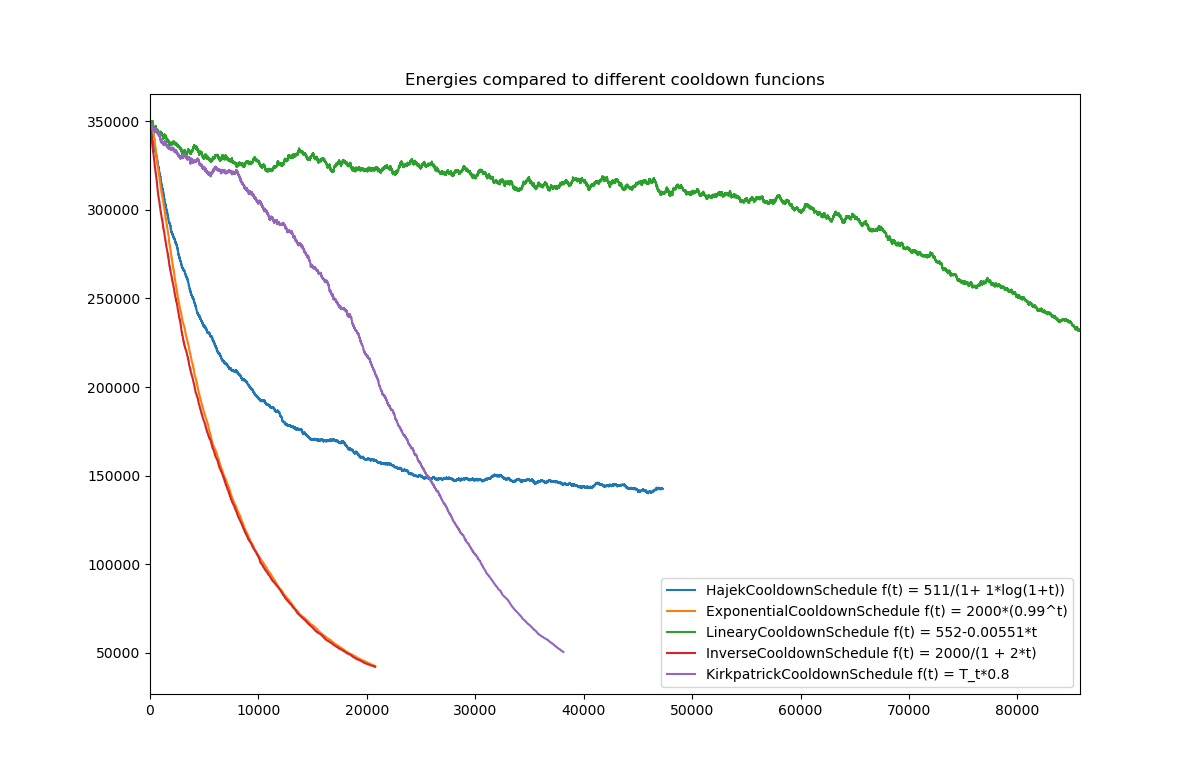
\includegraphics[width=\linewidth]{content/simulatedAnnealing/Bilder/Energy_Cooldown_compared_steps_85771.png}
    \caption{Vergleich von Abkühlfunktionen mit gesetzten Parametern
            alle mit 100000 Schritten; auf x-Achse sind erfolgreiche Schritte nach Wahrscheinlichkeitsakzeptanzfunktion
            aufgetragen}
    \label{pic:Cool Down Comparisson}
\end{figure}

%%%%%%%%%%%%%%%%%%%%%%%%%%%%%%%%%%%%%%%%%%%%%%%%%%%%%%%%%%%%%%%%%%%%%%%%%%%%%%%%%%%%%%%%%%%%%%%%%%%%%
%%%%%%%%%%%%%%%%%%%%%%% this is our cooling schedule we are going for %%%%%%%%%%%%%%%%%%%%%%%%%%%%%%%
%%%%%%%%%%%%%%%%%%%%%%%%%%%%%%%%%%%%%%%%%%%%%%%%%%%%%%%%%%%%%%%%%%%%%%%%%%%%%%%%%%%%%%%%%%%%%%%%%%%%%

\subsubsection{Kirkpatrick}
Wir haben uns bei unserem Optimierungsproblem für einen Abkühlvorgang, der in \cite{Kirkpatrick671} beschrieben wird, 
entschieden und in danach benannt. Die Abkühlfunktion hat hierbei exponentiellen Charakter. 

\begin{equation}\label{eq:ExponentialKirkpatrick}
  f(t) = T_0 * pow(\alpha,t)
\end{equation}

Wobei wieder $\alpha \in [0.8; 0.99]$ und nach Auflösung der Textur zu wählen ist. Ein anderer Parameter, der nach 
Auflösung der Textur zu wählen ist, ist das Quasi-Gleichgewicht. Mit dem Quasi-Gleichgewicht lässt sich erreichen, 
dass jeder Bildabschnitt vor dem jeweiligen Abkühlen jede Temperatur durchläuft und dabei jeden Bildabschnitt davor 
bewahrt in einen lokalen Minima zu verharren.
So lässt sich in einem direkten Vergleich mit dem bloßen exponentiellen Abkühlen in Abbildung 
\ref{pic:Cool Down Comparisson} erkennen, das wir anfangs langsamer abkühlen und immer wieder auch 
höhere Energiezustände bewusst zu lassen.

\begin{figure}[H]
    \centering
    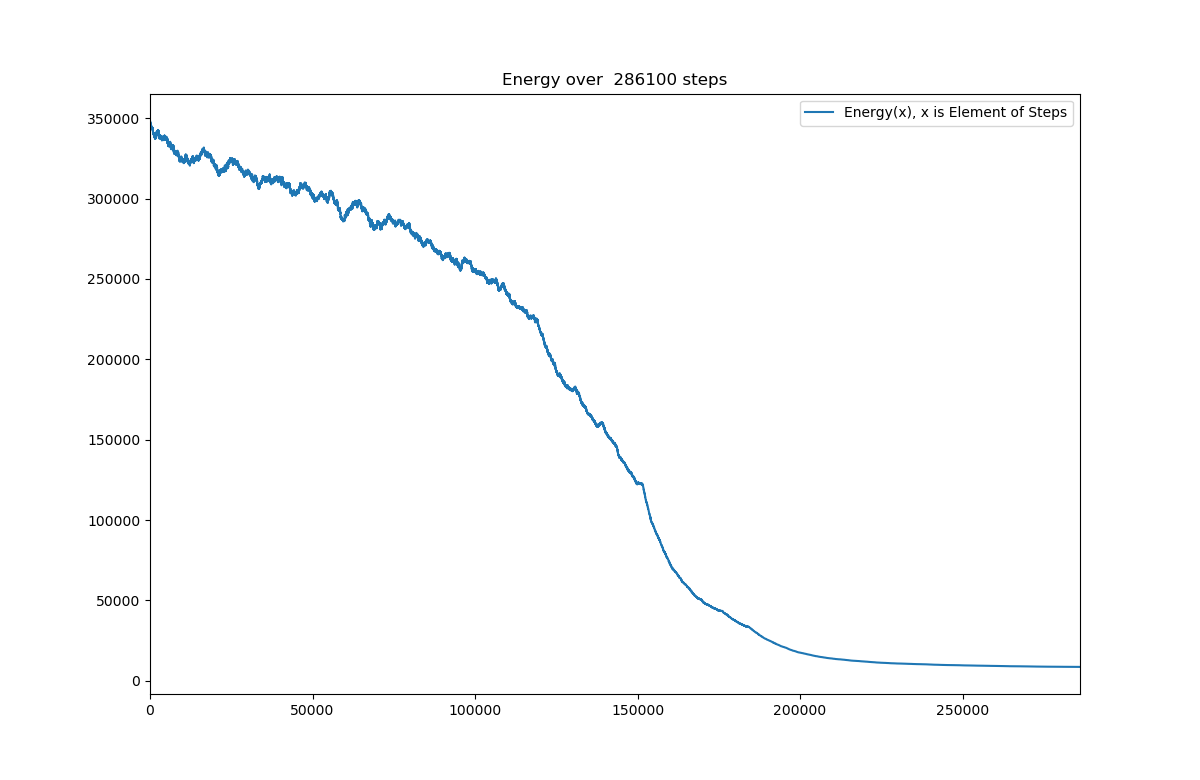
\includegraphics[width=\linewidth]{content/simulatedAnnealing/Bilder/Energy_286100_steps_KirkpatrickCooldownSchedule.png}
    \caption{Energieverlauf beim Simulated Annealing}
    \label{pic:kirkpatrick energie verlauf}
\end{figure}

Die Abbildung \ref{pic:kirkpatrick energie verlauf} verdeutlicht, dass wir durch unser Abkühlen insgesamt die 
Energiefunktion \ref{eq:pixel energy function} minimieren. Dabei akzeptieren wir in Abhängigkeit unserer Schritte,
anfangs sehr häufig und am Ende immer seltener, neben günstigeren Zuständen, auch energetische Höherwertigere.

\begin{figure}[H]
    \centering
    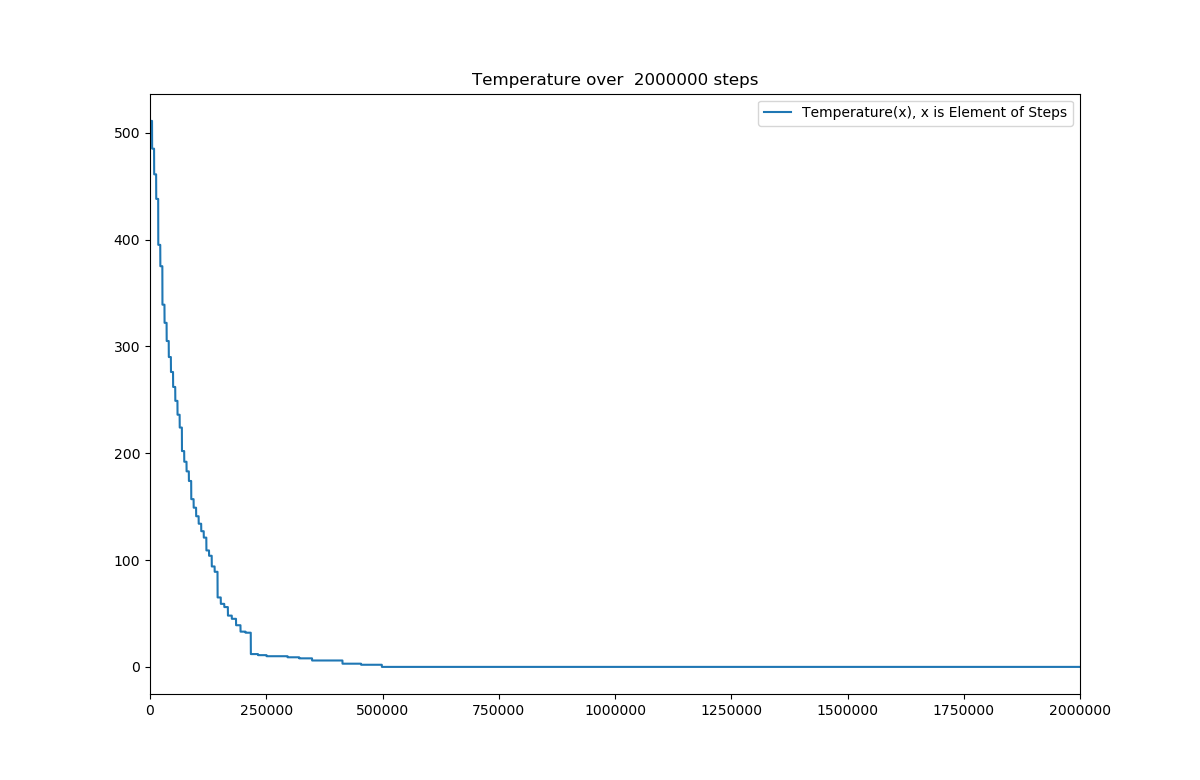
\includegraphics[width=\linewidth]{content/simulatedAnnealing/Bilder/Temperature.png}
    \caption{Temperaturverlauf}
    \label{pic:Temperaturverlauf kirkpatrick}
\end{figure}

Wir wählen die Starttemperatur (siehe Abbildung \ref{pic:Temperaturverlauf kirkpatrick}) folgendermaßen, dass 
anfangs alle Permutationen akzeptiert werden. Dazu muss die 
Akzeptanzwahrscheinlichkeitsfunktion \ref{eq:Akzeptanzwahrscheinlichkeitsfunktion} auch die energetisch
ungünstigste Permutation akzeptieren. Minimiere Argument der Exponentialfunktion \ref{fig:Exponentialfunktion}.
In unseren konkreten Fall: Maximales $\Delta_{Energy}$ bei einem 8-Bit Graustufenbild 2*255 = 510. Jeweilige 
Anpassungen müssen bei anderer Auflösung vorgenommen werden.

\begin{figure}[H]
    \centering
    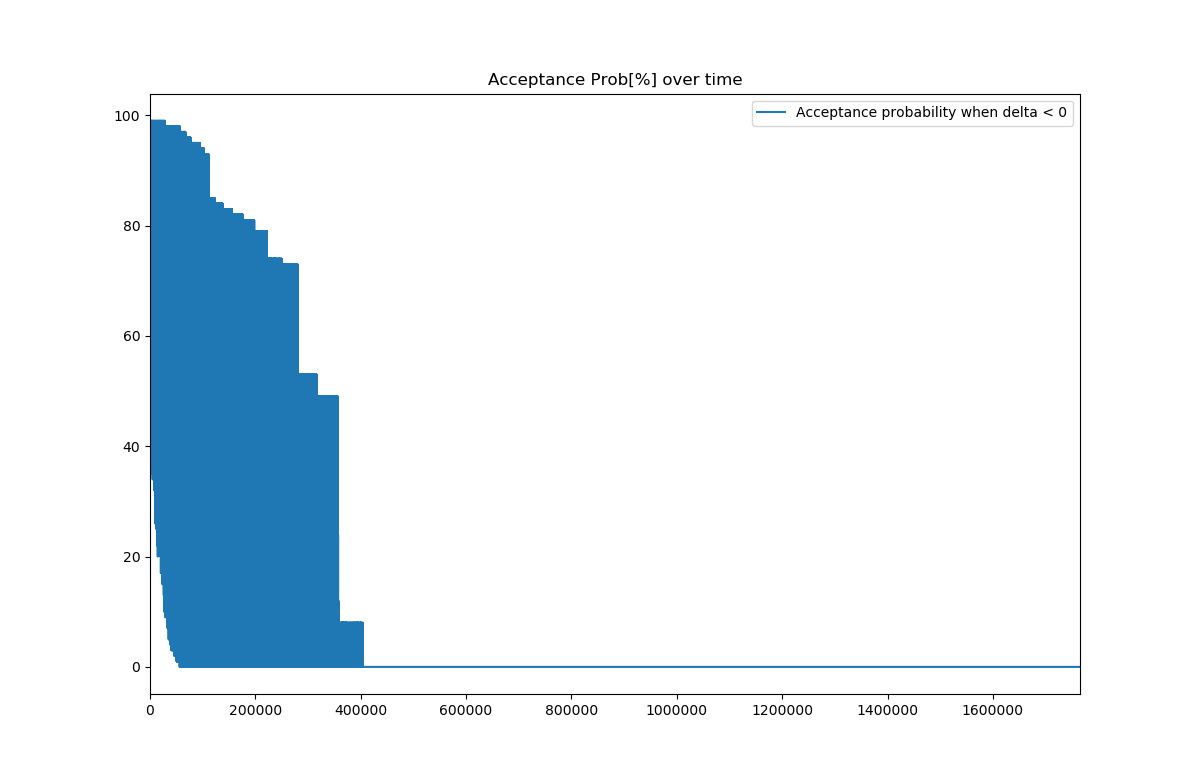
\includegraphics[width=\linewidth]{content/simulatedAnnealing/Bilder/Acceptance_Probabilities_over_time_1765297_steps_KirkpatrickCooldownSchedule.png}
    \caption{Akzeptanzfunktionsverlauf bei negativen Energiedeltas}
    \label{pic:Akzeptanzfunktionsverlauf kirkpatrick}
\end{figure}

Abbildung \ref{pic:Akzeptanzfunktionsverlauf kirkpatrick} zeigt das Aufkommen der Werte der Gleichung
\ref{eq:Akzeptanzwahrscheinlichkeitsfunktion} an. Zu Anfang gibt es keine niederen und ausschließlich 
hohe Wahrscheinlichkeiten der Akzeptanz wohingegen am Schluss keine energetisch schlechteren Permutationen 
akzeptiert werden.

\begin{figure}[H]
    \centering
    \begin{minipage}[t]{0.45\linewidth}
        \centering
        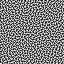
\includegraphics[interpolate=false,width=\linewidth]{content/simulatedAnnealing/Bilder/LDR_RGBA_0_64-RGBA_r_channel.png}
        \caption{Blue noise Textur 64x64}
    \end{minipage}
    \hfill
    \begin{minipage}[t]{0.45\linewidth}
        \centering
        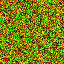
\includegraphics[interpolate=false,width=\linewidth]{content/simulatedAnnealing/Bilder/permutation_texture_295744_swapsKirkpatrickCooldownSchedule.png}
        \caption{Permutation; gespeichert in R,G-Channel einer PNG}
        \label{pic:Retargeting textur}
    \end{minipage}
\end{figure}

%%%%%%%%%%%%%%%%%%%%%%%%%%%%%%%%%%%%%%%%%%%%%%%%%%%%%%%%%%%%%%%%%%%%%%%%%%%%%%%%%%%%%%%%%%%%%%%%%%%%%%%%%%%%%%%%%%%%%%%%%%%%%%%%%%
%%%% Animate the annealing!!!!!! %%%%%%%%%%%%%%%%%%%%%%%%%%%%%%%%%%%%%%%%%%%%%%%%%%%%%%%%%%%%%%%%%%%%%%%%%%%%%%%%%%%%%%%%%%%%%%%%%
%%%%%%%%%%%%%%%%%%%%%%%%%%%%%%%%%%%%%%%%%%%%%%%%%%%%%%%%%%%%%%%%%%%%%%%%%%%%%%%%%%%%%%%%%%%%%%%%%%%%%%%%%%%%%%%%%%%%%%%%%%%%%%%%%%

\begin{figure}[H]

    \centering
    \begin{subfigure}[b]{0.2\linewidth}
      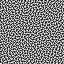
\includegraphics[width=\linewidth]{content/simulatedAnnealing/Bilder/Annealing/intermediate_applied_permutation_0_quasieqstepKirkpatrickCooldownSchedule_energy_348180-RGBA_r_channel.png}
       \caption{\nameref{ch:Content1:sec:blue noise} t}
       \label{pic:dither0}
    \end{subfigure}
    \begin{subfigure}[b]{0.2\linewidth}
      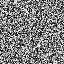
\includegraphics[width=\linewidth]{content/simulatedAnnealing/Bilder/Annealing/intermediate_applied_permutation_1_quasieqstepKirkpatrickCooldownSchedule_energy_313012-RGBA_r_channel.png}
      \caption{313012}
      \label{pic:abkühl_schritt_1}
    \end{subfigure}
    \begin{subfigure}[b]{0.2\linewidth}
      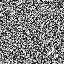
\includegraphics[width=\linewidth]{content/simulatedAnnealing/Bilder/Annealing/intermediate_applied_permutation_2_quasieqstepKirkpatrickCooldownSchedule_energy_281170-RGBA_r_channel.png}
      \caption{281170}
      \label{pic:abkühl_schritt_2}
    \end{subfigure}
    \begin{subfigure}[b]{0.2\linewidth}
        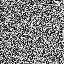
\includegraphics[width=\linewidth]{content/simulatedAnnealing/Bilder/Annealing/intermediate_applied_permutation_3_quasieqstepKirkpatrickCooldownSchedule_energy_253330-RGBA_r_channel.png}
         \caption{253330}
         \label{pic:abkühl_schritt_3}
      \end{subfigure}

    %%%%%%%%%%%%%%%%%%%%%%%%%%%%%%%%%%%%%%%%%%%%%%%%%%%%%%%%%%%%%%%%%%%%%%%%%%%%%%%%%%%%%%%%%%%%%%%%%%%%%%
    %%%%%%%%%%%%%%%%%%%%%%%%%%%%%%% second row
    %%%%%%%%%%%%%%%%%%%%%%%%%%%%%%%%%%%%%%%%%%%%%%%%%%%%%%%%%%%%%%%%%%%%%%%%%%%%%%%%%%%%%%%%%%%%%%%%%%%%%%

    \begin{subfigure}[b]{0.2\linewidth}
        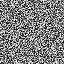
\includegraphics[width=\linewidth]{content/simulatedAnnealing/Bilder/Annealing/intermediate_applied_permutation_4_quasieqstepKirkpatrickCooldownSchedule_energy_185486-RGBA_r_channel.png}
        \caption{185486}
        \label{pic:abkühl_schritt_4}
    \end{subfigure}
    \begin{subfigure}[b]{0.2\linewidth}
        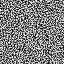
\includegraphics[width=\linewidth]{content/simulatedAnnealing/Bilder/Annealing/intermediate_applied_permutation_5_quasieqstepKirkpatrickCooldownSchedule_energy_136464-RGBA_r_channel.png}
        \caption{136464}
        \label{pic:abkühl_schritt_5}
    \end{subfigure}
    \begin{subfigure}[b]{0.2\linewidth}
        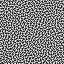
\includegraphics[width=\linewidth]{content/simulatedAnnealing/Bilder/Annealing/intermediate_applied_permutation_11_quasieqstepKirkpatrickCooldownSchedule_energy_29068-RGBA_r_channel.png}
         \caption{29068}
         \label{pic:abkühl_schritt_6}
    \end{subfigure}
    \begin{subfigure}[b]{0.2\linewidth}
        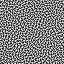
\includegraphics[width=\linewidth]{content/simulatedAnnealing/Bilder/Annealing/intermediate_applied_permutation_20_quasieqstepKirkpatrickCooldownSchedule_energy_13070-RGBA_r_channel.png}
        \caption{13070}
        \label{pic:abkühl_schritt_7}
    \end{subfigure}

    %%%%%%%%%%%%%%%%%%%%%%%%%%%%%%%%%%%%%%%%%%%%%%%%%%%%%%%%%%%%%%%%%%%%%%%%%%%%%%%%%%%%%%%%%%%%%%%%%%%%%%
    %%%%%%%%%%%%%%%%%%%%%%%%%%%%%%% third row
    %%%%%%%%%%%%%%%%%%%%%%%%%%%%%%%%%%%%%%%%%%%%%%%%%%%%%%%%%%%%%%%%%%%%%%%%%%%%%%%%%%%%%%%%%%%%%%%%%%%%%%

    \begin{subfigure}[b]{0.2\linewidth}
        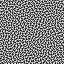
\includegraphics[width=\linewidth]{content/simulatedAnnealing/Bilder/Annealing/intermediate_applied_permutation_49_quasieqstepKirkpatrickCooldownSchedule_energy_8688-RGBA_r_channel.png}
        \caption{8688}
        \label{pic:abkühl_schritt_8}
    \end{subfigure}
    \begin{subfigure}[b]{0.2\linewidth}
        \begin{picture}(120,120)
            \put(35,50){\Huge $\approx$}
        \end{picture}
    \end{subfigure}
    \begin{subfigure}[b]{0.2\linewidth}
        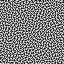
\includegraphics[width=\linewidth]{content/simulatedAnnealing/Bilder/next_dither_LDR_RGBA_0_64_r_channel.png}
        \caption{\nameref{ch:Content1:sec:blue noise} t+1}
        \label{pic:dither1}
    \end{subfigure}
    \caption{Der Prozess des Abkühlens mit jeweiliger Auswertung der Energiefunktion \ref{eq:pixel energy function}}
    \label{fig:annelaing animated}
    
  \end{figure}

  Nachdem wir in Bild 
  \begin{itemize}
    \item[\ref{pic:dither0}] unsere \nameref{ch:Content1:sec:blue noise} Textur zum Zeitpunkt t=0 
                              haben können wir in dem Bild
    \item[\ref{pic:abkühl_schritt_1}] typische Clusterbildungen erkennen, die die Folge von 
                                    uniformen randomisierten Vertauschungen sind. Diese hatte wir bereits 
                                    im Abschnitt \ref{ch:Content1:sec:blue noise} und \ref{ch:Content1:sec:Quasi-Zufallsfolgen}
                                    besprochen. Diese Vertauschungen sind die Folge der hohen Temperatur, welche wiederrum zur Folge haben, 
                                    dass alle Vertauschungen von der Funktion \ref{eq:Akzeptanzwahrscheinlichkeitsfunktion} angenommen werden. 
                                    Die Bilder  
    \item[\ref{pic:abkühl_schritt_2}-\ref{pic:abkühl_schritt_4}] sind die Folge der abnehmenden Temperatur und der daraus folgenden geringeren 
                                    Akzeptanz schlechterer, energiereicherer Zustände. Bessere Zustände werden allerdings immer angenommen und 
                                    daher die immer bessere \nameref{ch:Content1:sec:blue noise} Verteilung. Die bessere Verteilung ist eben über 
                                    die gesamte Textur zu erkennen. Mit abnehmender Energie in den Bildern   
    \item[\ref{pic:abkühl_schritt_5}-\ref{pic:abkühl_schritt_8}] lassen wir sehr wenige/keine schlechteren Zustände mehr zu und gelangen durch 
                                    lokale Permutationen zu einer immer exakteren Verteilung.  
    \item[\ref{pic:dither1}] Zieltextur; so soll unsere Textur t nach angewandter 
                              Permutation aussehen. 
  \end{itemize}





